\documentclass[11pt]{beamer}

 \usepackage[utf8]{inputenc}
 \usepackage[T1]{fontenc}
 \usepackage{palatino}

\usepackage{polski}
\usepackage{subfig}
\usepackage{tikz}
\usepackage{amsmath}

\usetheme{Boadilla}

\title[MO -- Projekt]{%
	MO -- Projekt \vspace{0.5cm}\\%
	Zbrojenie
}

\author[Skibiński, Kaźmieruk]{Maksymilian Skibiński, Paweł Kaźmieruk}

\date{\today{} r.}

\graphicspath{{./img/}}

\captionsetup[subfigure]{labelformat = empty}

%\mode<presentation>
%{
%	\setbeamercovered{transparent}
%	% or whatever (possibly just delete it)
%}

\begin{document}

\frame{\titlepage}



\begin{frame}{Zadanie}{Prostokątny fundament}
\begin{figure}[h!]
	\centering
	\includegraphics[height = 0.32 \linewidth]{img9}
\end{figure}
\end{frame}

\begin{frame}{Zadanie}{Zbrojenie}
\begin{figure}[h!]
	\centering
	
\includegraphics[height = 0.32 \linewidth]{img2}
\end{figure}
\end{frame}

\begin{frame}{Zadanie}{Zbrojenie -- uproszczenie}
\begin{figure}[h!]
	\centering
	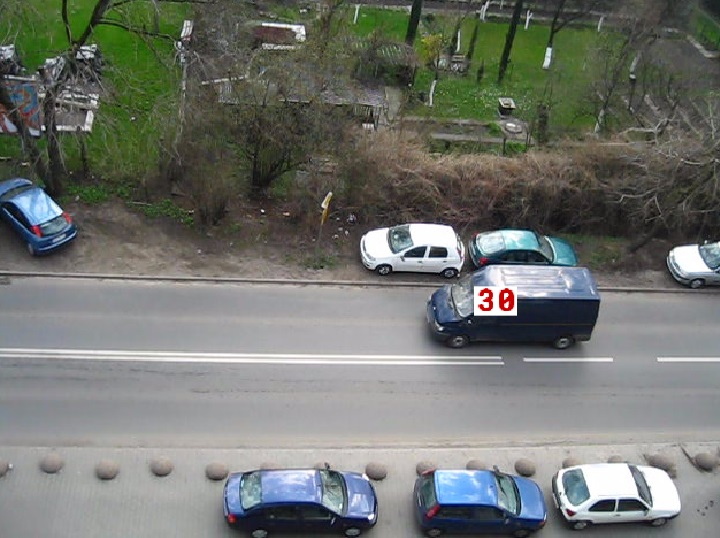
\includegraphics[height = 0.32\linewidth]{img4}
\end{figure}
\end{frame}

\begin{frame}{Zadanie}{Sklep}
Oferta sklepu:
\begin{itemize}
\item<1-> możemy kupować druty o rozmiarze $e$ [m],
\item<2-> możemy je także ciąć dowolną ilość razy w dowolnych miejscach.
\end{itemize}

\vspace{0.5cm}

\pause\pause

Wszystko oczywiście kosztuje:
\begin{itemize}
\item[ ] cena za metr pręta: $g$ [zł],
\item[ ] cena za jedno cięcie: $h$ [zł].
\end{itemize}
\end{frame}

\begin{frame}{Zadanie}{Pozostałe informacje}
\begin{itemize}
\item<1-> Transport prętów wymaga, by wszystkie pręty były niedłuższe niż $f$ [m],
\item<2-> Jeśli do budowy jednego pręta na siatce fundamentowej użyjemy więcej niż jednego pręta, to należy zastosować ,,zakładkę'' o minimalnej długości $i$ [m].
\end{itemize}
\end{frame}

\begin{frame}{Zadanie}{Podsumowanie}
Wszystkie parametry:
\begin{itemize}
\item<1-> $a$ x $b$ [m] -- wymiary fundamentu,
\item<2-> $c$ x $d$ [m] -- wymiary ,,oczka'' siatki,
\item<3-> $e$ -- rozmiar sprzedawanych prętów,
\item<6-> $f$ -- ograniczenie transportowe,
\item<4-> $g$ -- koszt jednego metra pręta,
\item<5-> $h$ -- koszt jednego cięcia,
\item<7-> $i$ -- długość minimalnej zakładki.
\end{itemize}
\end{frame}

\begin{frame}{Zadanie}{Podsumowanie}
Dostaliśmy także pewne przykładowe wartości tych parametrów:
\begin{itemize}
\item[ ] $a$ x $b$ = 8 m x 8 m,
\item[ ] $c$ x $d$ = 0.2 m x 0.15 m,
\item[ ] $e$ = 6 m,
\item[ ] $f$ = 4 m,
\item[ ] $g$ = 2.08 zł,
\item[ ] $h$ = 0.2 zł,
\item[ ] $i$ = 0.3 m.
\end{itemize}
\end{frame}


\begin{frame}
\begin{center}
\LARGE Opis matematyczny
\end{center}
\end{frame}


\begin{frame}{Pręty}{Kupno}
\begin{itemize}
\item Możemy kupować pręty $e$ metrowe,
\item ale możemy je także ciąć w dowolnych miejscach dowolną ilość razy.
\end{itemize}

\begin{figure}[h!]
	\centering
	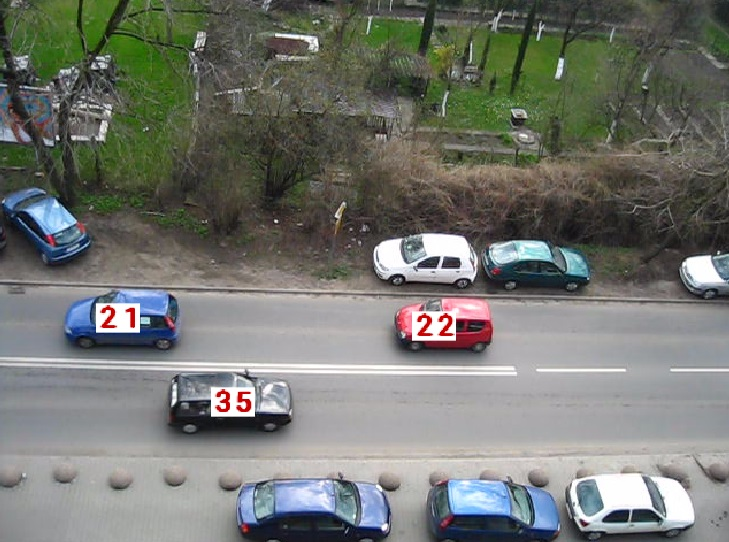
\includegraphics[width = 0.4 \linewidth]{img1}
\end{figure}
\end{frame}

\begin{frame}{Pręty}{Zapis wektorowy}
W ten sposób, wszystkie pręty, które posiadamy możemy opisywać w postaci wektorów:
\begin{align*}
\mathbf{p}_1 = & \left[p_{11} \ p_{12} \ \cdots \ p_{1i} \ \cdots \ p_{1Y_1}\right] \\
\mathbf{p}_2 = & \left[p_{21} \ p_{22} \ \cdots \ p_{2i} \ \cdots \ p_{2Y_2}\right] \\
& \vdots \\
\mathbf{p}_j = & \left[p_{j1} \ p_{j2} \ \cdots \ p_{ji} \ \cdots \ p_{jY_j}\right] \\
& \vdots \\
\mathbf{p}_U = & \left[p_{U1} \ p_{U2} \ \cdots \ p_{Ui} \ \cdots \ p_{UY_U}\right] \\
\end{align*}

\begin{itemize}
\item<2-> Jest w sumie $U$ prętów,
\item<3-> Każdy pręt $p_j$ składa się z $Y_j$ części.
\end{itemize}
\end{frame}


\begin{frame}{Pręty}{Zapis macierzowy}
Ewentualnie, można też zapisać wszystko w postaci jednej większej macierzy:
\begin{equation*}
\mathbf{P} =
\begin{bmatrix}
p_{11} & p_{12} & \cdots & p_{1i} & \cdots & p_{1Y} \\
p_{21} & p_{22} & \cdots & p_{2i} & \cdots & p_{2Y} \\
\vdots & \vdots & \vdots & \vdots & \vdots & \vdots \\
p_{j1} & p_{j2} & \cdots & p_{ji} & \cdots & p_{jY} \\
\vdots & \vdots & \vdots & \vdots & \vdots & \vdots \\
p_{U1} & p_{U2} & \cdots & p_{Ui} & \cdots & p_{UY}
\end{bmatrix}
\end{equation*}

\pause

Ale, tym razem musiałby być ustalony pewien stały wymiar $Y$.
\end{frame}

\begin{frame}{Pręty}{Ograniczenia}
Na pręty oraz ich części (,,podpręty'') nałożone są ograniczenia:
\begin{itemize}
\item<1-> Długość całego pręta to $e$ m, ze względu na sklep, zatem jego składowe muszą w sumie dawać $e$ m:
\begin{equation*}
\forall_{k \in \{1, 2, ..., U\}} \quad \sum_{j = 1}^{Y_k} p_{kj} = e
\end{equation*}

\item<2-> Każda składowa każdego prętu musi być krótsza niż $f$ m, ze względu na transport:
\begin{equation*}
\forall_{k \in \{1, 2, ..., U\}} \ \forall_{j \in \{1, 2, ..., Y_k\}} \quad
p_{kj} \le f
\end{equation*}
\end{itemize}
\end{frame}

\begin{frame}{Funkcja celu}
Zatem, jako że chcemy minimalizować wydane pieniądze:
\begin{equation*}
\text{min} \leftarrow J = U \cdot e \cdot g + \sum_{j = 1}^{U} (Y_j - 1) \cdot h
\end{equation*}

gdzie:
\begin{itemize}
\item[ ] $U$ -- liczba prętów,
\item[ ] $Y_j$ -- liczba ,,podprętów'',
\item[ ] $e$ -- długość sprzedawanych prętów,
\item[ ]
\item[ ] $g$ -- cena za metr pręta,
\item[ ] $h$ -- cena za jedno przecięcie.
\end{itemize}
\end{frame}



\begin{frame}{Siatka}
Cała siatka składa się z wielu prętów i wygląda mniej więcej tak:
\begin{figure}[h!]
	\centering
	
\includegraphics[height = 0.32 \linewidth]{img2}
\end{figure}
\end{frame}

\begin{frame}{Siatka}
Cała siatka składa się z wielu prętów i wygląda mniej więcej tak:
\begin{figure}[h!]
	\centering
	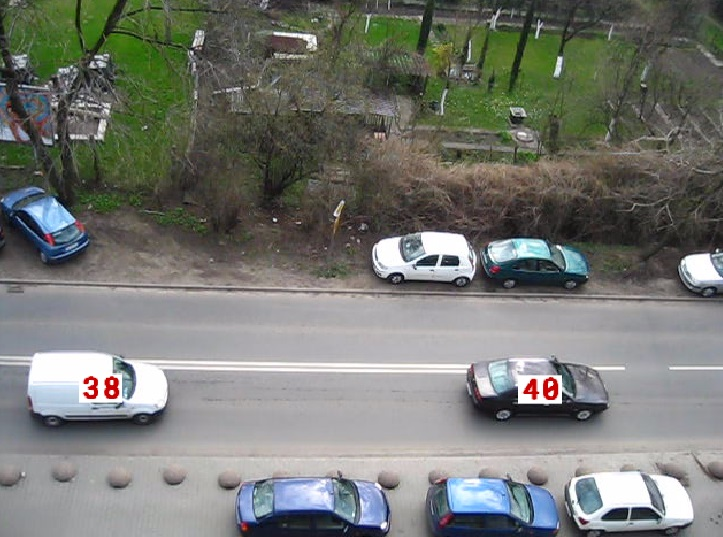
\includegraphics[height = 0.32 \linewidth]{img3}
\end{figure}

Weźmy pod uwagę jeden pręt.
\end{frame}


\begin{frame}{Siatka}{Zakładki}
\begin{figure}[h!]
	\centering
	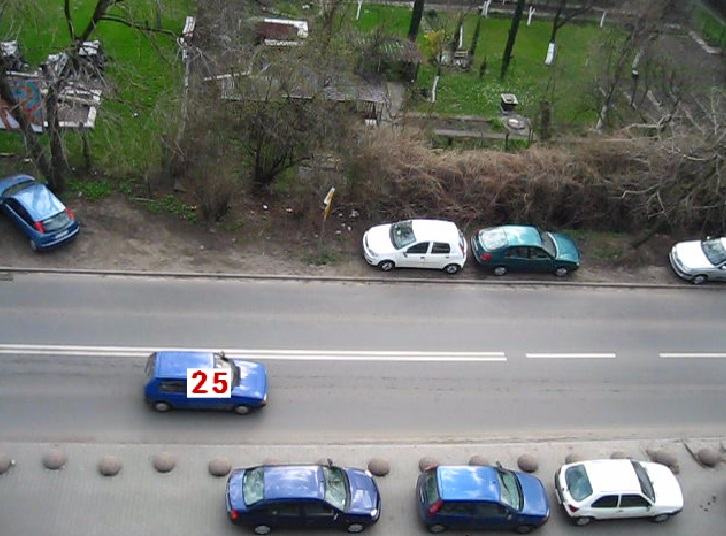
\includegraphics[width = 0.5\linewidth]{img5}
\end{figure}

\begin{itemize}
\item<1-> Jeśli mamy jeden pręt... to OK,
\item<2-> Jeśli kładziemy więcej niż jeden pręt stosujemy zakładkę o pewnej minimalnej długości,
\item<3-> równie dobrze zakładka może być dłuższa,
\item<4-> więcej prętów to więcej zakładek.
\end{itemize}
\end{frame}

\begin{frame}{Siatka}{Zakładki}
Spójrzmy na zakładkę od innej strony -- rozsuńmy pręty:
\begin{figure}[h!]
	\centering
	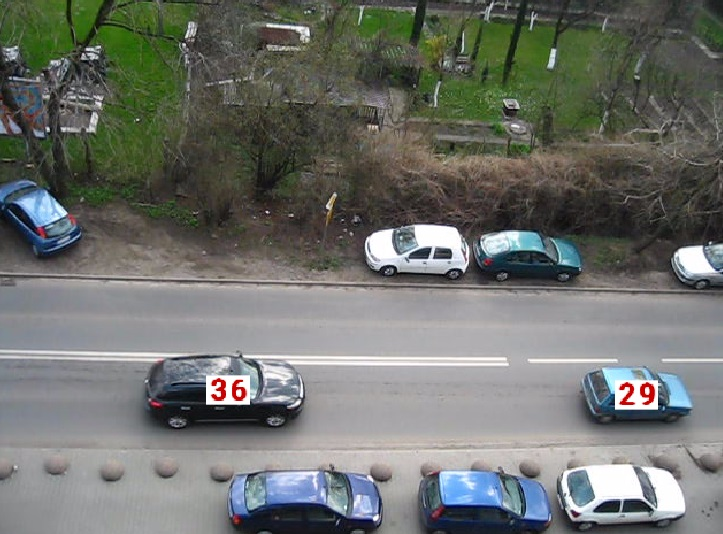
\includegraphics[width = 0.75\linewidth]{img6}
\end{figure}

\pause

Czym więcej prętów, tym ich wspólna długość musi być większa.

\end{frame}


\begin{frame}{Siatka}{Równanie stanu}
Jeden pręt na siatce możemy opisać poprzez równanie stanu.

\pause

\begin{align*}
x_{n+1} = x_n + u_n \quad & \\
& x_0 = 0 \\
& x_N  \ge a + (N - 1) \cdot 2 \cdot i \\
& i \le u_n \le f
\end{align*}

gdzie:
\begin{itemize}
\item[ ] $a$ -- to długość wymiaru siatki,
\item[ ] $N$ -- to liczba prętów na długości,
\item[ ] $i$ -- to długość minimalnej zakładki,
\item[ ] $f$ -- to ograniczenie transportowe.
\end{itemize}
\end{frame}

\begin{frame}{Siatka}{Równania stanu}
Każdy pręt z siatki jest opisanie przez swój stan i sterowania:
\begin{figure}[h!]
	\centering
	\includegraphics[width = 0.75\linewidth]{img7}
\end{figure}

\pause

Jest w sumie $M$ prętów:
\begin{itemize}
\item $R$ poziomych,
\item $M - R$ pionowych.
\end{itemize}
\end{frame}

\begin{frame}{Siatka}{Sterowania}
Wektory sterowań dla każdego prętu siatki:
\begin{align*}
\mathbf{u}_1 &= \left[ u_{10} \ u_{11} \ \cdots \ u_{1K_1} \right] \\
\mathbf{u}_2 &= \left[ u_{20} \ u_{21} \ \cdots \ u_{2K_2} \right] \\
& \vdots \\
\mathbf{u}_i &= \left[ u_{i0} \ u_{i1} \ \cdots \ u_{iK_i} \right] \\
& \vdots \\
\mathbf{u}_M &= \left[ u_{M0} \ u_{M1} \ \cdots \ u_{MK_M} \right] \\
\end{align*}

\pause

Analogicznie do prętów zakupionych ($p$) te zapisy też możemy sprowadzić do jednej macierzy $\mathbf{U}$.
\end{frame}

\begin{frame}{Siatka}{Podsumowanie}
Równanie stanu:
\begin{equation*}
x_{in+1} = x_{in} + u_{in}
\end{equation*}

\pause

Ograniczenia na stan:
\begin{equation*}
x_{i0} = 0 \qquad
x_{iN_i} \ge
	\begin{cases}
	a + (N_i - 1) \cdot 2 \cdot i \qquad \text{dla} \ i \in \{1, 2, \ldots, R\} \\
	b + (N_i - 1) \cdot 2 \cdot i \qquad \text{dla} \ i \in \{R+1, R+2, \ldots, M\}
	\end{cases}
\end{equation*}

\pause

Ograniczenie na sterowania to:
\begin{equation*}
i \le u_{in} \le f,
\end{equation*}

czyli pręty muszą być dłuższe niż minimalna zakładka ($i$), ale krótsze niż ograniczenie transportowe ($f$).

\end{frame}

\begin{frame}{Powiązanie}
Zaproponowaliśmy opisy dwóch zagadnień:
\begin{itemize}
\item prętów zakupionych (wektory $p$),
\item prętów na siatce (wektory $u$).
\end{itemize}

\pause

Jak to powiązać?
\end{frame}

\begin{frame}{Powiązanie}
Zasada:
\begin{equation*}
\forall_{p_{ij}} \ \exists!_{u_{mk}} \ p_{ij} = u_{mk}
\qquad \land \qquad
\forall_{u_{mk}} \ \exists!_{p_{ij}} \ u_{mk} = p_{ij}
\end{equation*}

\vspace{0.5cm}

\begin{center}
Dla każdego pręta $p_{ij}$ (zakupionego) istnieje \\ dokładnie jeden pręt $u_{mk}$ (zbrojeniowy) i vice versa.
\end{center}
\end{frame}

\begin{frame}{Powiązanie}
Zakładając macierzowy zapis $\mathbf{P}$ i $\mathbf{U}$:
\begin{figure}[h!]
	\centering
	\includegraphics[width = 0.8\linewidth]{img8}
\end{figure}
\end{frame}

\begin{frame}
Niestety, sposób w jaki opisaliśmy problem utrudnił nam znalezienie rozwiązania...
\end{frame}

\begin{frame}
\begin{center}
\LARGE Koniec
\end{center}
\end{frame}



\end{document}